% Left analytic data panel; right exact group counts and two prediction rules.
% Volume three architecture figures. Independent export only; not book fonts.
\colorlet{MutedBlueFill}{FigureBlueFill}
\colorlet{MutedGreenFill}{FigureGreenFill}
\colorlet{MutedPurple}{FigurePurple}
\colorlet{MutedPurpleFill}{FigurePurpleFill}
\tikzset{
 v3 picture/.style={x=1mm,y=1mm,font=\figurefont\fontsize{8}{10}\selectfont,text=FigureInk,line width=.65pt},
 v3 box/.style={draw=FigureBlue,fill=white,rounded corners=1.8pt,line width=.7pt,inner sep=2.5pt,align=center},
 v3 data/.style={v3 box,fill=FigureBlueFill},
 v3 model/.style={v3 box,draw=FigureGreen,fill=FigureGreenFill},
 v3 output/.style={v3 box,draw=FigureYellow,fill=FigureYellowFill},
 v3 risk/.style={v3 box,draw=FigureRed,fill=FigureRedFill},
 v3 group/.style={draw=FigureBlue,rounded corners=1.8pt,line width=.65pt,inner sep=3mm},
 v3 flow/.style={draw=FigureStroke,line width=.75pt,-{Stealth[length=1.65mm,width=1.05mm]},rounded corners=1pt},
 v3 guide/.style={draw=FigureMuted,line width=.6pt,dashed},
 v3 feedback/.style={v3 flow,draw=FigureGreen,dashed},
 v3 title/.style={draw=none,fill=none,font=\figurefont\fontsize{8}{10}\selectfont,align=center,inner sep=1pt},
 v3 note/.style={draw=none,fill=none,font=\FigureNoteFont\fontsize{7.5}{9.5}\selectfont,text=FigureMuted,align=center,inner sep=1pt},
 v3 label/.style={draw=none,fill=none,font=\figurefont\fontsize{8}{10}\selectfont,align=center,inner sep=1pt},
 v3 wire/.style={draw=FigureMuted,line width=.45pt},
 v3 point/.style={circle,draw=FigureBlue,fill=FigureBlueFill,minimum size=2.3mm,inner sep=0pt,line width=.55pt}
}
% Bring pre-existing native TikZ geometry to the same typography and scale.
\tikzset{
 foundation picture/.append style={font=\figurefont\fontsize{8}{10}\selectfont,line width=.65pt},
 foundation node/.append style={rounded corners=1.8pt,line width=.7pt,font=\figurefont\fontsize{8}{10}\selectfont},
 foundation heading/.append style={draw=none,fill=none,font=\figurefont\fontsize{8}{10}\selectfont},
 foundation note/.append style={draw=none,fill=none,font=\FigureNoteFont\fontsize{7.5}{9.5}\selectfont},
 foundation flow/.append style={line width=.75pt,-{Stealth[length=1.65mm,width=1.05mm]}},
 foundation frame/.append style={rounded corners=1.8pt,line width=.7pt},
 foundation edge label/.append style={draw=none,fill=none,font=\figurefont\fontsize{8}{10}\selectfont}
}
% Official Lucide outline icons, consistently used across diagrams. Size in mm.
\newcommand{\VIcon}[5]{\node[inner sep=0pt] at (#2,#3) {\includegraphics[width=#4mm]{figures/03-foundations/00-shared/tikz/icons/#1-#5.pdf}};}
% A neutral network glyph (not a claim about an actual model architecture).
% Coordinates denote its centre; scale 1 gives 13 x 8 mm.
\newcommand{\VNet}[4]{\begin{scope}[shift={(#1,#2)},scale=#3]
 \foreach \a in {-3,0,3}{\foreach \b in {-3,0,3}{\draw[v3 wire] (-5,\a)--(0,\b);}}
 \foreach \a in {-3,0,3}{\draw[v3 wire] (0,\a)--(5,0);}
 \foreach \a in {-3,0,3}{\draw[draw=#4,fill=#4,line width=.55pt] (-5,\a) circle(.9);\draw[draw=#4,fill=white,line width=.55pt] (0,\a) circle(.9);}
 \draw[draw=#4,fill=#4,line width=.55pt] (5,0) circle(.9);
\end{scope}}
\newcommand{\VDots}[4]{\foreach \k in {0,1,2,3}{\fill[#4] ({#1+2.7*\k},#2) circle(#3);}}
% Feature vector/tensor elements are scientific glyphs, not decorative icons.
\newcommand{\VVector}[4]{\foreach \k in {0,...,4}{\fill[#4,rounded corners=.25pt] ({#1+2.2*\k},#2) rectangle ++(1.5,#3);}}

\begin{tikzpicture}[v3 picture]
\path[use as bounding box] (0,0) rectangle (163.2,84);
\node[inner sep=0pt] at (29,43) {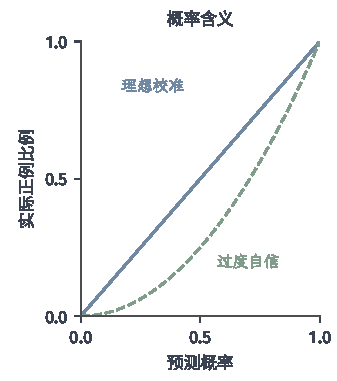
\includegraphics[width=57mm]{figures/03-foundations/03-trustworthiness/tikz/trust-calibration-discrimination/assets/panel.pdf}};
\node[v3 title] at (86,79) {组1：$20\%$ 正例};
\node[v3 title] at (137,79) {组2：$80\%$ 正例};
\node[v3 box,minimum width=43mm,minimum height=22mm] (g1) at (86,64) {};
\node[v3 box,minimum width=43mm,minimum height=22mm] (g2) at (137,64) {};
% Ten identical person glyphs per equal-size group; a blue fill denotes a positive.
\foreach \g/\base/\positives in {1/72/2,2/123/8}{
 \foreach \k in {0,...,9}{
  \pgfmathtruncatemacro{\col}{mod(\k,5)}
  \pgfmathtruncatemacro{\row}{int(\k/5)}
  \pgfmathsetmacro{\x}{\base+7*\col}
  \pgfmathsetmacro{\y}{68-9*\row}
  \ifnum\k<\positives\def\personfill{FigureBlue}\else\def\personfill{white}\fi
  \draw[draw=FigureStroke,fill=\personfill,line width=.55pt] (\x,\y+2) circle(1.4);
  \path[draw=FigureStroke,fill=\personfill,line width=.55pt,rounded corners=.6pt] (\x-2.2,\y-2.8)--(\x-2.2,\y-1.4) arc[start angle=180,end angle=0,radius=2.2]--(\x+2.2,\y-2.8)--cycle;
 }
}
\node[v3 title] at (112,43) {常数预测};
\node[v3 label] (c1) at (92,34) {$p=0.5$};
\node[v3 label] (c2) at (131,34) {$p=0.5$};
\draw[v3 flow,draw=FigureBlue] (86,53)--(86,46)--(92,46)--(c1.north);
\draw[v3 flow,draw=FigureBlue] (137,53)--(137,46)--(131,46)--(c2.north);
\node[v3 title] at (112,21) {分组预测};
\node[v3 label] (p1) at (92,11) {$p=0.2$};
\node[v3 label] (p2) at (131,11) {$p=0.8$};
\draw[v3 flow,draw=FigureGreen] (68,53)--(68,11)--(p1.west);
\draw[v3 flow,draw=FigureGreen] (156,53)--(156,11)--(p2.east);
\end{tikzpicture}
